\section{Diagramm mit LibreOffice Draw}
\hon{}

Ein \textit{ERD} wird in \textit{LibreOffice Draw} korrekt und vollständig erzeugt. Alle Sonderfälle wie unter anderem \textit{Abhängige Entity-Typen}, \textit{Super-Sub-Beziehungstypen} und \textit{mehrwertige Beziehungen} werden bei der Generierung aller Datenmodelle (siehe Kapitel \ref{cha:Testmodelle}) in der erwünschten Form dargestellt.

\subsection{Probleme bei der Darstellung}

Bei der Erstellung eines \textit{ERDs} sind folgende Probleme aufgetreten:
\begin{itemize}
	\item In \textit{LibreOffice Draw} gibt es keine vorhandene Möglichkeit die \textit{Krähenfußnotation} zu implementieren, da keine vordefinierte Formen für die Elemente dieser Notation vorhanden sind. Ein manuelles Erzeugen der Elemente ist komplex und aufwendig.
	\item Bei dem Layout, dass mittels \textit{graphviz-layout} generiert wird, kann es zu, je nach Datenmodell, ein oder mehreren Überschneidungen kommen. Ein solcher Vorfall beeinträchtigt die Lesbarkeit des \textit{ERDs}.
	Die Abbildung \ref{überschneidung} zeigt eine Überschneidung der \textit{Konnektoren} bei dem Datenmodell \textit{SIS}.
\end{itemize}
\noindent
\begin{figure}[H]
	\begin{center}
		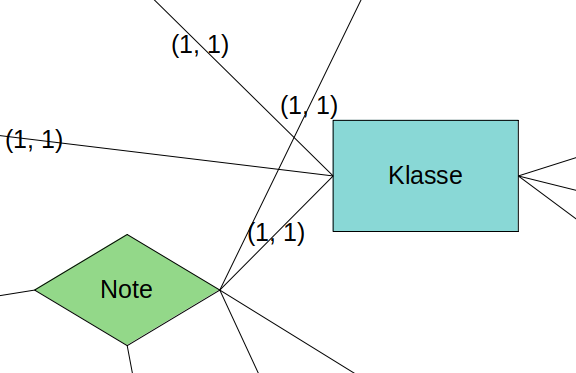
\includegraphics[width=10cm]{images/19.png}
		\caption{Überschneidung der \textit{Konnektoren} bei dem Datenmodell \textit{SIS}}
		\label{überschneidung}
	\end{center}
\end{figure}

\subsection{Beispiel eines ER-Diagramms in LibreOffice Draw}
\hon{}

In der Abbildung \ref{LODERD} wird das \textit{ERD} des Datenmodells \textit{Weingut} gezeigt. Dieses wurde vollständig durch das Tool erzeugt und wurde händisch \textbf{nicht} nachbearbeitet.

\begin{figure}[H]
	\begin{center}
		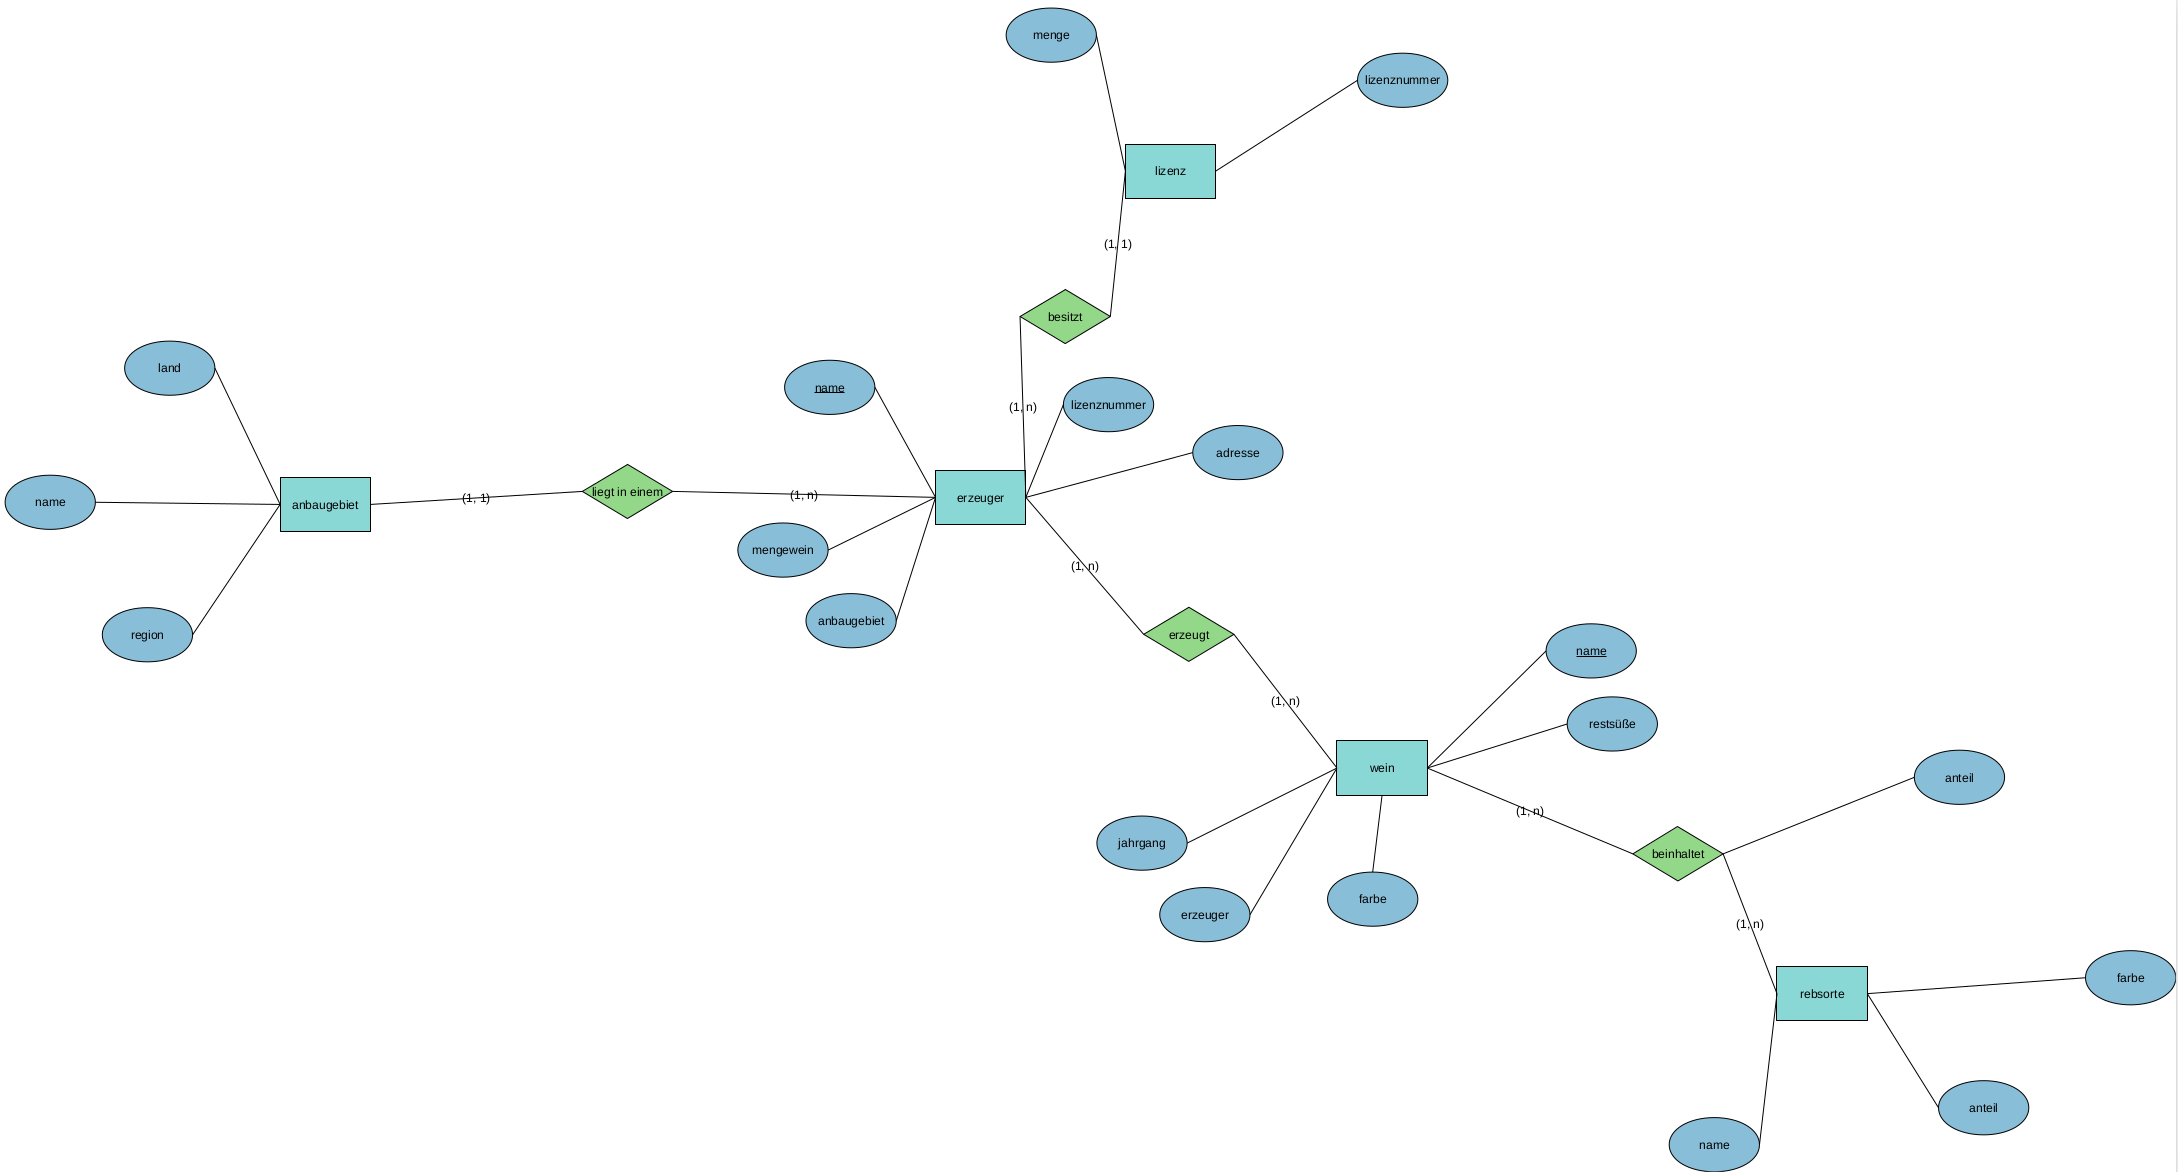
\includegraphics[width=14cm]{images/20.png}
		\caption{ER-Diagramm des Datenmodells \textit{Weingut}}
		\label{LODERD}
	\end{center}
\end{figure}